\documentclass{article}
\usepackage[utf8]{inputenc}
\usepackage{graphicx}

\title{Penanganan Error}
\author{itsmeakil707 }
\date{October 2019}

\begin{document}
\title{Penanganan Error}
\author{Akil Munawwar \\ 1184041 \\ D4 TI 1B}
\maketitle

\section{Peringatan Error}
    \begin{enumerate}
        \item Syntax Error adalah kesalahan ketika menulis suatu kode yang tidak sesuai dengan kaidah bahasa pemrograman tersebut. Cara menanganinya ialah dengan memperbaiki penulisan kode yang salah tersebut.
        \item Zero Division Error adalah kesalahan yang dilakukan ketika menjumlahkan suatu angka dengan angka 0. Cara menanganinya ialah dengan tidak membagi angka tersebut dengan angka 0.
        \item IdentationError adalah kesalahan yang dilakukan saat menulis kode python dengan satu baris tanpa ada nya jarak. Cara menanganinya ialah dengan memberi space atau tab pada yang error tersebut.
    \end{enumerate}
\section{TryExcept}
    \begin{enumerate}
        \item File 2err.py
        \begin{figure}[!htbp]
            \centering
            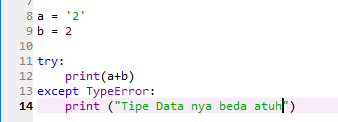
\includegraphics{TipeDataError.PNG}
            \caption{Tipe Data Yang Beda}
        \end{figure}
    \end{enumerate}
\end{document}
